Obtido o valor de $x$ que define a posição (profundidade) da linha neutra, é possível verificar em que domínio a peça atingirá o Estado Limite Último. Na flexão simples, que está sendo considerada, os domínios possíveis são 2, 3 e 4. No início do domínio 2 tem-se $\epsilon_c=0$, e no final do domínio 4, $\epsilon_s=0$, que são as piores situações que podem ocorrer (um dos dois materiais não contribui na resistência). O melhor é que a peça trabalhe no domínio 3; o domínio 2 é aceitável; e o domínio 4 deve ser evitado. Cabe então a pergunta: Conhecido o momento e demais variáveis necessárias para resolver o problema, como saber se a seção está trabalhando no domínio 3 e se a armadura já atingiu a deformação de escoamento? É possível saber por meio da relação entre as deformações e a posição da linha neutra.

\begin{figure}[H]
	\begin{center}
	\caption{Domínios de deformação.}
    	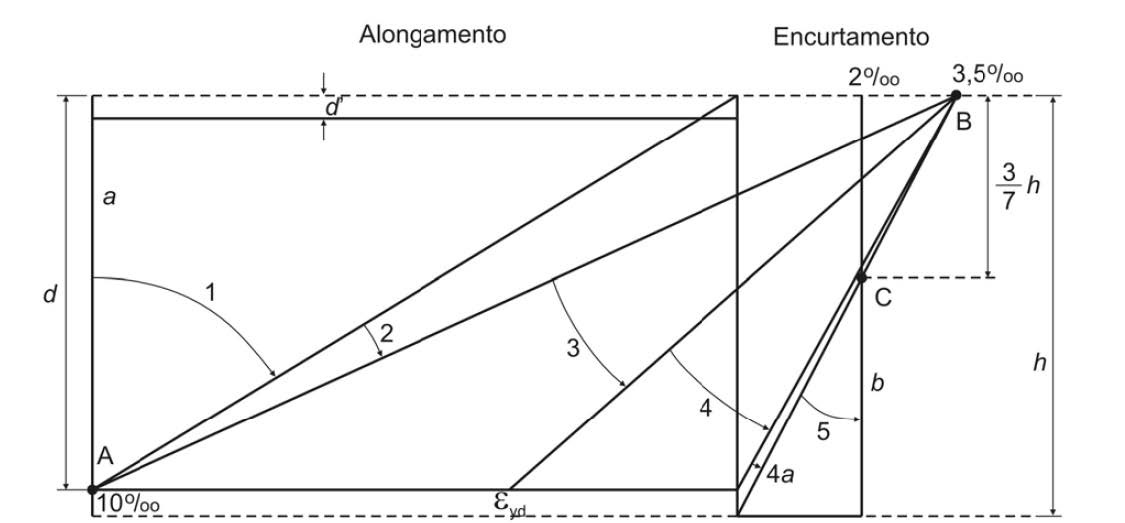
\includegraphics[width=\textwidth]{Linha-neutra/Imagens/Dominios-de-deformacao.jpg}
	\end{center}
\end{figure}

A linha neutra no domínio 1 está em ($-\infty<x\leqslant0$); no domínio 2 é necessário encontrar por semelhança de triângulos, já que foi considerada a hipótese de que as seções permanecem planas após as deformações. Ou seja:
$$\frac{x}{3,5\text{\textperthousand}}=\frac{d-x}{10\text{\textperthousand}}$$
$$10\text{\textperthousand}\cdot x=3,5\text{\textperthousand}\cdot d-3,5\text{\textperthousand}\cdot x$$

Isolando $x$, tem-se:
$$x=\frac{3,5\text{\textperthousand}\cdot d}{10\text{\textperthousand}+3,5\text{\textperthousand}}=0,259\cdot d$$

Portanto, a linha neutra do domínio 2 está em ($0<x\leqslant0,259\cdot d$). De maneira semelhante, para o domínio 3, tem-se:
\begin{equation}
	\label{equacao-dominio-3}
	\frac{x}{3,5\text{\textperthousand}}=\frac{d-x}{\epsilon_s}
\end{equation}

Pela Lei de Hooke ($\sigma=\text{E}\cdot\epsilon$) e pelo módulo de Young do aço ser de 210 $GPa$, o valor de $\epsilon_s$ (valor de deformação onde ocorre o início do escoamento do aço) depende do tipo de aço utilizado. O mais comum nas contruções de concreto armado é o aço CA-50. O número 50 diz que a tensão de escoamento desse aço é de 50 $kN/{cm}^2$. Aplicando a Lei de Hooke para esse aço, tem-se:
$$50\;\frac{kN}{{cm}^2}=21000\;\frac{kN}{{cm}^2}\cdot\epsilon_k$$
$$\epsilon_k=\frac{50\;\frac{kN}{{cm}^2}}{21000\;\frac{kN}{{cm}^2}}=2,38\text{\textperthousand}$$

O valor de $\epsilon_s=2,38\text{\textperthousand}/1,15=2,07\text{\textperthousand}$. Portanto, desenvolvendo e isolando $x$ na Equação~\eqref{equacao-dominio-3} para o aço CA-50, tem-se:
$$\frac{x}{3,5\text{\textperthousand}}=\frac{d-x}{2,07\text{\textperthousand}}$$
$$2,07\text{\textperthousand}\cdot x=3,5\text{\textperthousand}\cdot d-3,5\text{\textperthousand}\cdot x$$
$$x=\frac{3,5\text{\textperthousand}\cdot d}{2,07\text{\textperthousand}+3,5\text{\textperthousand}}=0,628\cdot d$$

Portanto, a linha neutra do domínio 3 está em ($0,259\cdot d<x\leqslant0,628\cdot d$). Para o domínio 4 e para o aço CA-50, a linha neutra está em ($0,628\cdot d<x\leqslant d$); no domínio 4a, está em ($d<x\leqslant h$) e por último, no domínio 5, está em ($h<x<\infty$).
